
\section{Interazioni fra componenti}
\label{sec:Interazioni}
\subsection{Costruzione del grafo della mappa topologica}

\begin{figure}[H]
	\centering
	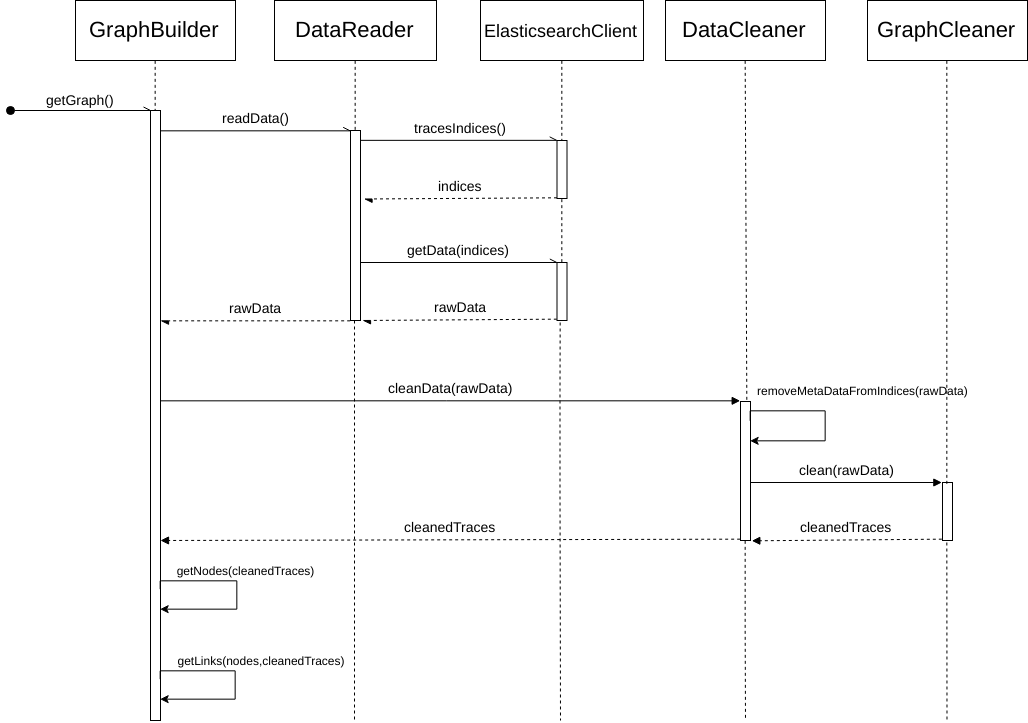
\includegraphics[width=1\textwidth]{Images/DiagrammaSequenzaGraph.png}
	\caption{Diagramma di Sequenza UML rappresentante la costruzione del grafo della mappa topologica}
	\label{img:seqGraph}
\end{figure}

Un'istanza di \texttt{GraphBuilder} richiama il metodo \texttt{readData()} su un oggetto \texttt{DataReader} che si occupa prima di selezionare gli indici dell'istanza di Elasticsearch che hanno al loro interno delle traces tramite la funzione \texttt{tracesIndices()} e successivamente di effettuare una richiesta per ogni indice recuperato al fine di recupera i dati associati.
Ricevuti i dati, viene invocato il metodo \texttt{cleanData()} passandogli come parametro i dati, che si occupa della pulizia dei dati superflui provenienti da Elasticsearch tramite la funzione \texttt{removeDataFromIndices()}. Tramite la funzione \texttt{clean()} invece vengono puliti i dati superflui alla costruzione della mappa topologica attraverso un'istanza di \texttt{GraphCleaner}.
In seguito alla pulizia dei dati, l'istanza di \texttt{GraphBuilder} costruisce l'insieme dei nodi che faranno parte della mappa topologica tramite \texttt{getNodes()} e l'insieme di collegamenti che ci saranno tra i nodi del grafo tramite \texttt{getLink()}, lavorando sul'istanza di \texttt{Graph} al suo interno.


\subsection{Costruzione dei dati della stack trace}
\begin{figure}[H]
	\centering
	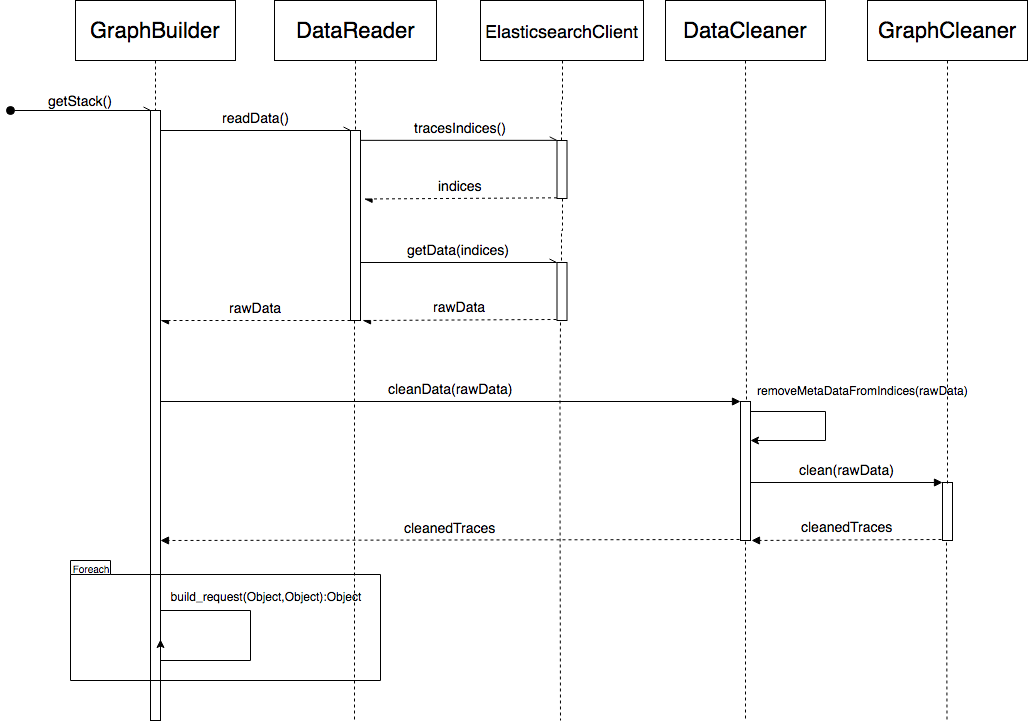
\includegraphics[width=1\textwidth]{Images/DiagrammaSequenzaStack.png}
	\caption{Diagramma di Sequenza UML rappresentante la costruzione della stack trace}
	\label{img:seqGraph}
\end{figure}
La sequenza di azioni per quanto riguarda l'interazione tra \texttt{StackBuilder}, \texttt{DataReader}, \texttt{ElasticsearchClient}, \texttt{DataCleaner} e \texttt{StackCleaner} è uguale a quella riguardande \texttt{GraphBuilder.}\\
Dopo aver ricevuto i dati e averli ripuliti dai dati superflui \texttt{StackBuilder} utilizza i metodi \texttt{build\_request()} e \texttt{build\_pageload\_request()} per ottenere la struttura ottimale per la costruzione delle richieste da visualizzare nella stack trace.


\section{Tracciamento dei requisiti}
\label{sec:Tracciamento}
Qui swego 
